\documentclass[a4paper, 10pt, conference]{ieeeconf}  
%\documentclass[letterpaper, 10 pt, conference]{ieeeconf}  % Use this for US paper
\IEEEoverridecommandlockouts
\overrideIEEEmargins
\bibliographystyle{IEEEtran}
%\usepackage{natbib}

\usepackage{graphicx}  % Add graphics capabilities
\usepackage{color}
\usepackage{amsmath} % assumes amsmath package installed
\usepackage{amssymb}  % assumes amsmath package installed
\usepackage{mathrsfs}
%\usepackage{amsthm}
\usepackage{epstopdf}
\newtheorem{theorem}{Theorem}
\newtheorem{lemma}{Lemma}
\newtheorem{definition}{Definition}
\newcommand{\jo}{(j\omega)}
\newcommand{\jok}{(e^{-j\omega_k})}
\newcommand{\jro}{(e^{-j\omega},\rho)}
\newcommand{\jrok}{(e^{-j\omega_k},\rho)}



\title{A Data-Driven Loop-Shaping Approach to Design Controllers for Power Converters} 
% Title, preferably not more than 10 words.


\author{Achille Nicoletti$^{1}$ and Michele Martino$^{1}$ and Alireza Karimi$^{2}$% <-this % stops a space
\thanks{*This work was not supported by any organization}% <-this % stops a space
\thanks{$^{1}$Achille Nicoletti and Michele Martino are both with the European Organization for Nuclear Research (CERN), 
 CH-1211 Geneva 23, Switzerland
        {\tt\small  e-mail: achille.nicoletti@cern.ch / michele.martino@cern.ch}}%
\thanks{$^{2}$Alireza Karimi is with Ecole Polytechnique F\'{e}d\'{e}rale de Lausanne (EPFL), Institute of Mechanical Engineering (IGM),
   CH-1015 Lausanne, Switzerland
        {\tt\small e-mail: alireza.karimi@epfl.ch}}%
}

%\thanks[footnoteinfo]{Sponsor and financial support acknowledgment
%goes here. Paper titles should be written in uppercase and lowercase
%letters, not all uppercase.}

%\author[First]{Achille Nicoletti} 
%\author[First]{Michele Martino} 
%\author[Second]{Alireza Karimi}

%\address[First]{The European Organization for Nuclear Research (CERN), 
  % CH-1211 Geneva 23, Switzerland (e-mail: achille.nicoletti@cern.ch / michele.martino@cern.ch)}
%\address[Second]{Ecole Polytechnique F\'{e}d\'{e}rale de Lausanne (EPFL), 
   %CH-1015 Lausanne, Switzerland (e-mail: alireza.karimi@epfl.ch)}


\begin{document}

\maketitle
\thispagestyle{empty}
\pagestyle{empty}

\begin{abstract}                % Abstract of not more than 250 words.
A new loop-shaping data-driven approach is presented for synthesizing controllers for the CERN power converter control system. This method uses the frequency response function (FRF) of a system in order to avoid the problem of unmodeled dynamics associated with parametric models. For this particular application, it is shown that a convex optimization problem can be formulated (in either the $H_\infty$ or $H_2$ sense) to shape the closed-loop FRF while guaranteeing the closed-loop stability. This optimization problem is realized by linearizing a non-convex constraint around a stabilizing operating point. The effectiveness of the method is illustrated by designing a controller for the SATURN power converter which is used in the Large Hadron Collider, in injector machines, and for pulsed applications at CERN. Experimental validation in the time domain is also presented. 
\end{abstract}


%===============================================================================
\section{Introduction}
Today's industrial processes pose challenging problems to control engineers due to the increasing complexities of system structures. In order to simplify the controller design process, these systems are approximated with low-order models; this reduces both time and effort in synthesizing a controller. However, this approximation can create stability and performance problems since these low-order models are subject to model uncertainty. Data-driven control methods seek to alleviate this problem by synthesizing controllers based on time-domain or frequency-domain data (i.e., synthesis is model independant). A survey on the differences associated with model-based control and data-driven control has been addressed in \cite{HW13} and \cite{BCE12}; the authors assert that model-based control methods are inherently less robust due to the unmodeled dynamics of a process, and that these controllers are unsafe for practical applications. In other words, the parametric uncertainties and the unmodeled dynamics associated with the data-driven scheme are irrelevant, and the only source of uncertainty is the measurement noise. 

Data-driven controllers can be synthesized either on-line or off-line; the on-line methods such as the classical direct adaptive control (MRAC) \cite{LLMK11}, model-free adaptive control (MFAC) \cite{HJ13}, and the unfalsified control (UC) \cite{ST97} methodologies design controllers using time-domain data. Iterative feedback tuning (IFT) \cite{Hja02}, correlation-based tuning (CBT) \cite{KMB02a}, virtual reference feedback tuning (VRFT) \cite{CLS02}, non-iterative data-driven model reference control \cite{KVB07} methodologies are all off-line time-domain data-driven methods.  The widely used PID controller are usually tuned based on a set of time-domain or frequency-domain data. 

Frequency-domain based controller synthesis methods are design schemes that continue to spark the interest of many researchers. The authors in \cite{KNND13b} establish a robust frequency-domain controller design methods that requires a solution to a non-linear optimization problem. A frequency-domain loop-shaping method for fixed-structure controllers is proposed in \cite{KNND13c}; however, stability is not guaranteed with this method and must be verified a posteriori. Controller synthesis methods belonging to the $\mathcal{H}_{\infty}$ control framework minimizes the $\mathcal{H}_{\infty}$ norm of a weighted closed-loop sensitivity function. A convex optimization approach is used to design linearly-parameterized (LP) controllers with loop shaping and $\mathcal{H}_{\infty}$ performance in \cite{KG10}. This method is extended to multiple-input multiple-output (MIMO) systems for computing decoupling LP-MIMO controllers in \cite{GKL10b}. In \cite{NK14}, this method of designing LP controllers was further extended to MIMO systems with delay. Recently, the necessary and sufficient conditions for the existence of $\mathcal{H}_{\infty}$ controllers for SISO systems represented by their frequency response has been proposed in \cite{KNZ16}.

The proposed method in this paper invokes a new data-driven control design scheme for a specific power converter application at CERN. Currently, the load (i.e., the magnet of the particle accelerator) is approximated as a simple first-order system (series $RL$ circuit); however, as shown in \cite{GB65}, the parameters of the magnet are frequency dependent. Additionally, it has been shown in \cite{KZ98} that the vacuum chamber of the magnet is also frequency dependent (due to the skin depth effect and the chamber geometry). Therefore, it is appropriate to consider a data-driven based design to regulate the power converter control system.  In this work, it is shown that a loop-shaping design in the $\mathcal{H}_\infty$ or $\mathcal{H}_2$ sense can be formulated through a convex optimization problem; however, the methods described in this paper can also be applied to mixed $\mathcal{H}_2$ and $\mathcal{H}_\infty$ problems (i.e., minimizing the norm of weighted sensitivity functions). Additionally, with certain conditions on the controller parameters, it is shown that the closed-loop stability is guaranteed. 

The paper is organized as follows. The class of models represented by FRF's are addressed in section \ref{sec:prelim}. Section \ref{sec:system} discusses the framework of the power converter control system and its functionality at CERN. The main results and theoretical bases are addressed in section \ref{sec:main}; in this section, loop-shaping constraints are formulated for the power converter control system. Section \ref{sec:case} is dedicated to a case study where the effectiveness of the method is demonstrated by applying the proposed design scheme to a power converter control system for a specific accelerator requirement. Finally, the concluding remarks are given in section \ref{sec:conclusion}.

\section{Preliminaries}
\label{sec:prelim}
The class of systems discussed in this paper will be Linear Time-Invariant Single-Input Single-Output (LTI-SISO) systems that will be represented by a FRF $G\jo$.  The FRF can be obtained directly with a given transfer function (TF) model, or through an identification experiment using the Fourier analysis method. Let $U\jo$ and $Y\jo$ represent the FRF's of the system input and output signals, respectively. Then the FRF of the system can be represented as 
\begin{equation}
G\jo = Y\jo U^{-1}\jo
\end{equation}
If the data is noisy, then $G\jo$ is characterized as the Empirical Transfer Function Estimate (ETFE) and is asymptotically unbiased \cite{Lju99}. For such systems, a multiplicative uncertainty can be considered to ensure robustness in the presence of noise perturbations. In general, a set $\mathcal{G}$ can be formulated to represent a plant model containing $p$ FRF models:
\begin{equation}
\mathcal{G} = \{G_l\jo; \quad l=1,\ldots,p; \quad \forall \omega \in \Omega\}
\end{equation} 
$\Omega \in [0,\infty)$. For simplicity, one model from the set $\mathcal{G}$ will be considered, and the subscript $l$ will be omitted. However, in general, the design procedures outlined in this paper can be applied to the multi-model case. 

Additionally, for notation purposes, let us define $\mathscr{S}$ as the set of all strictly proper (stable) TF's and $\mathscr{P}$ as the set of all proper (stable) TF's. 

\section{System Framework}
\label{sec:system}
\begin{figure}
\centering
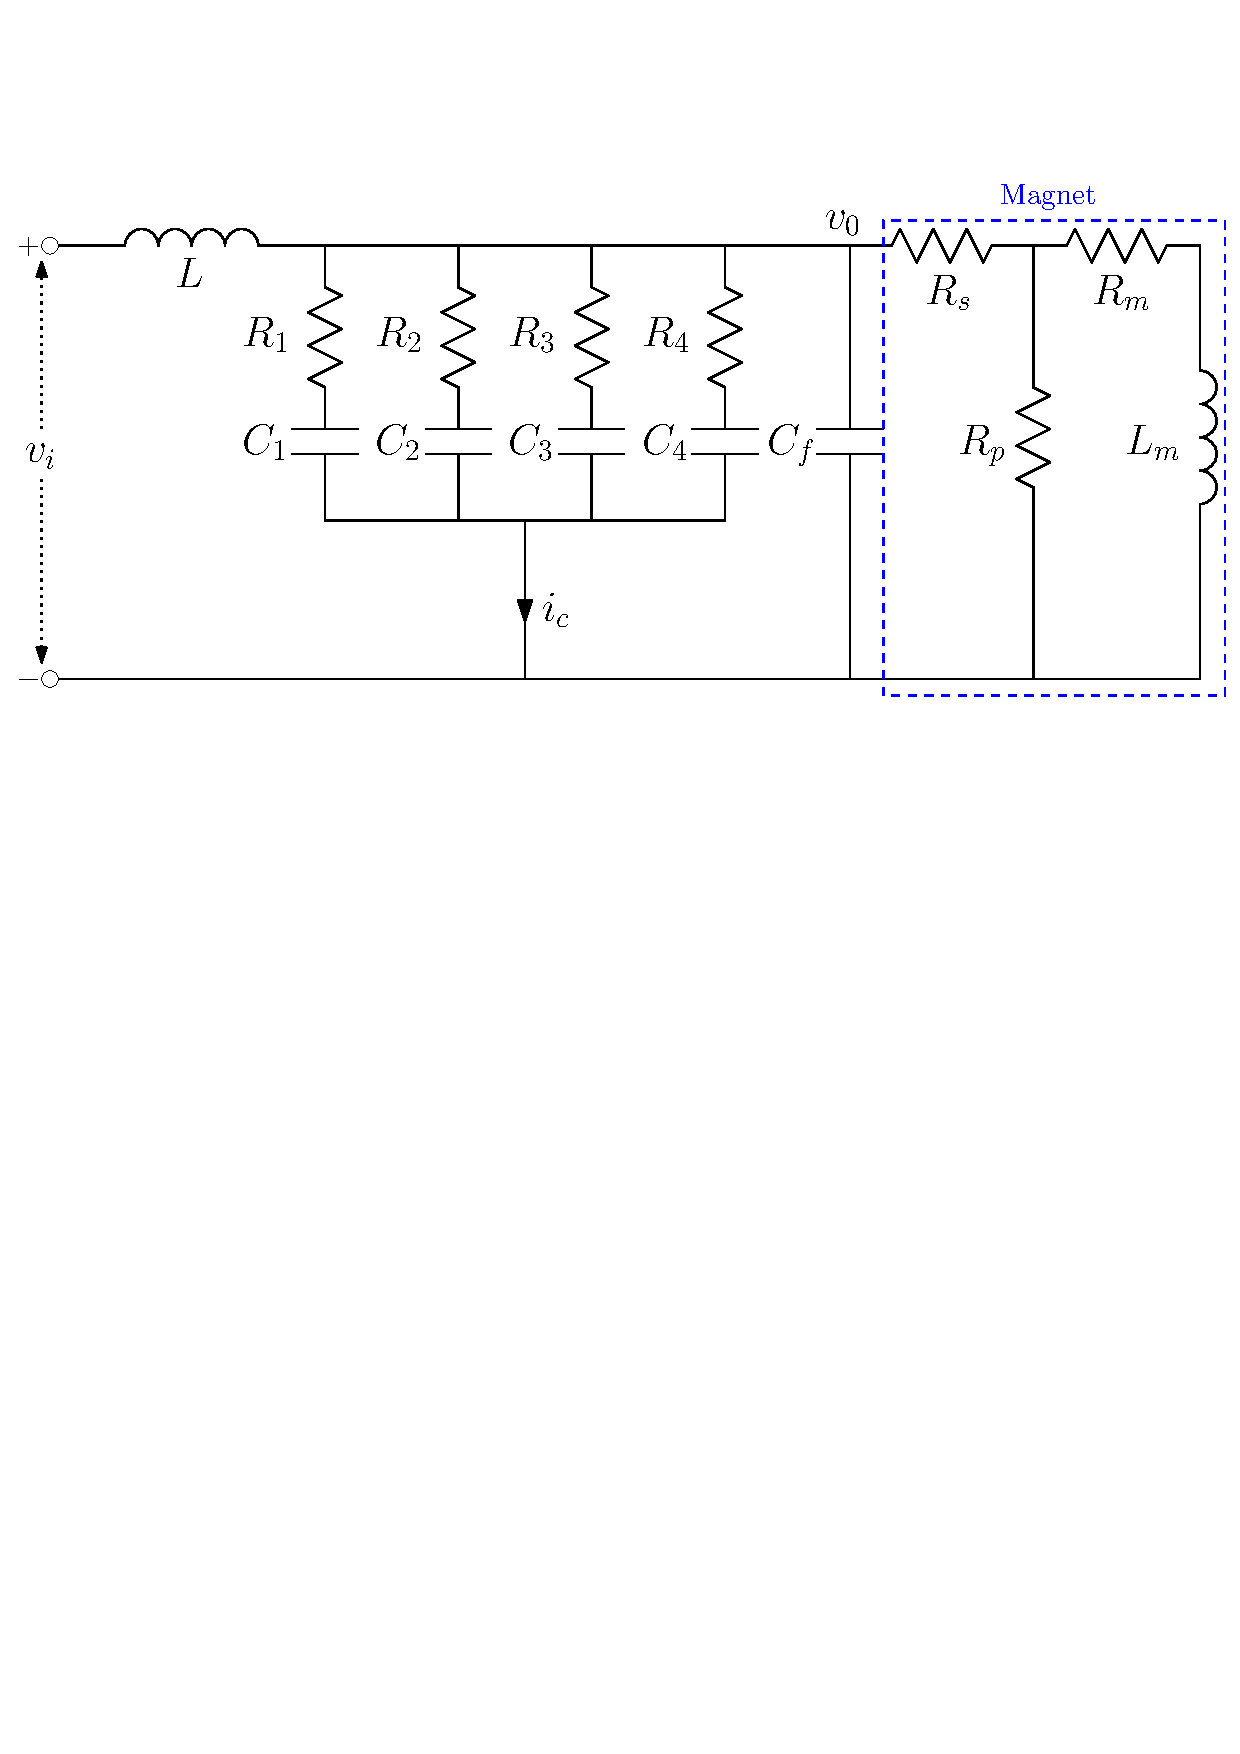
\includegraphics[width=\columnwidth]{../pics/circuit_partial_a}
\caption{Power converter filter schematic (from $v_i$ to $v_0$). The magnet represents the load of the process.}
\label{fig:circuit}
\end{figure}
The power converter voltage source filter has the structure shown in Fig.~\ref{fig:circuit}. The input voltage $v_i$ is the output of a pulse-width modulated signal (which will be discussed in more detail in section \ref{sec:case}). The TF from $v_i$ to $v_0$ describes the filter of the power converter. The magnet (i.e., the load) is connected to the output of the converter. For general applications at CERN, the objective is to control the current in the magnet (through $L_m$) such that the error between this output current and a delayed version of the reference current is minimized. However, the objective of this paper is to design and implement a controller to shape the FRF between the reference voltage and $v_0$. This intermediate control is performed due to the fact that the power converter typically possesses large resonances, and a controller is required to attenuate these resonances in order to ensure better performance in the current loop. Another reason for implementing this type of control structure at CERN is for commissioning purposes; if/when faults occur in the system, each loop can be verified one at a time to ensure quality operation.

The system structure for this application is shown in Fig.~\ref{fig:damping_loop}. 
\begin{figure}
\centering
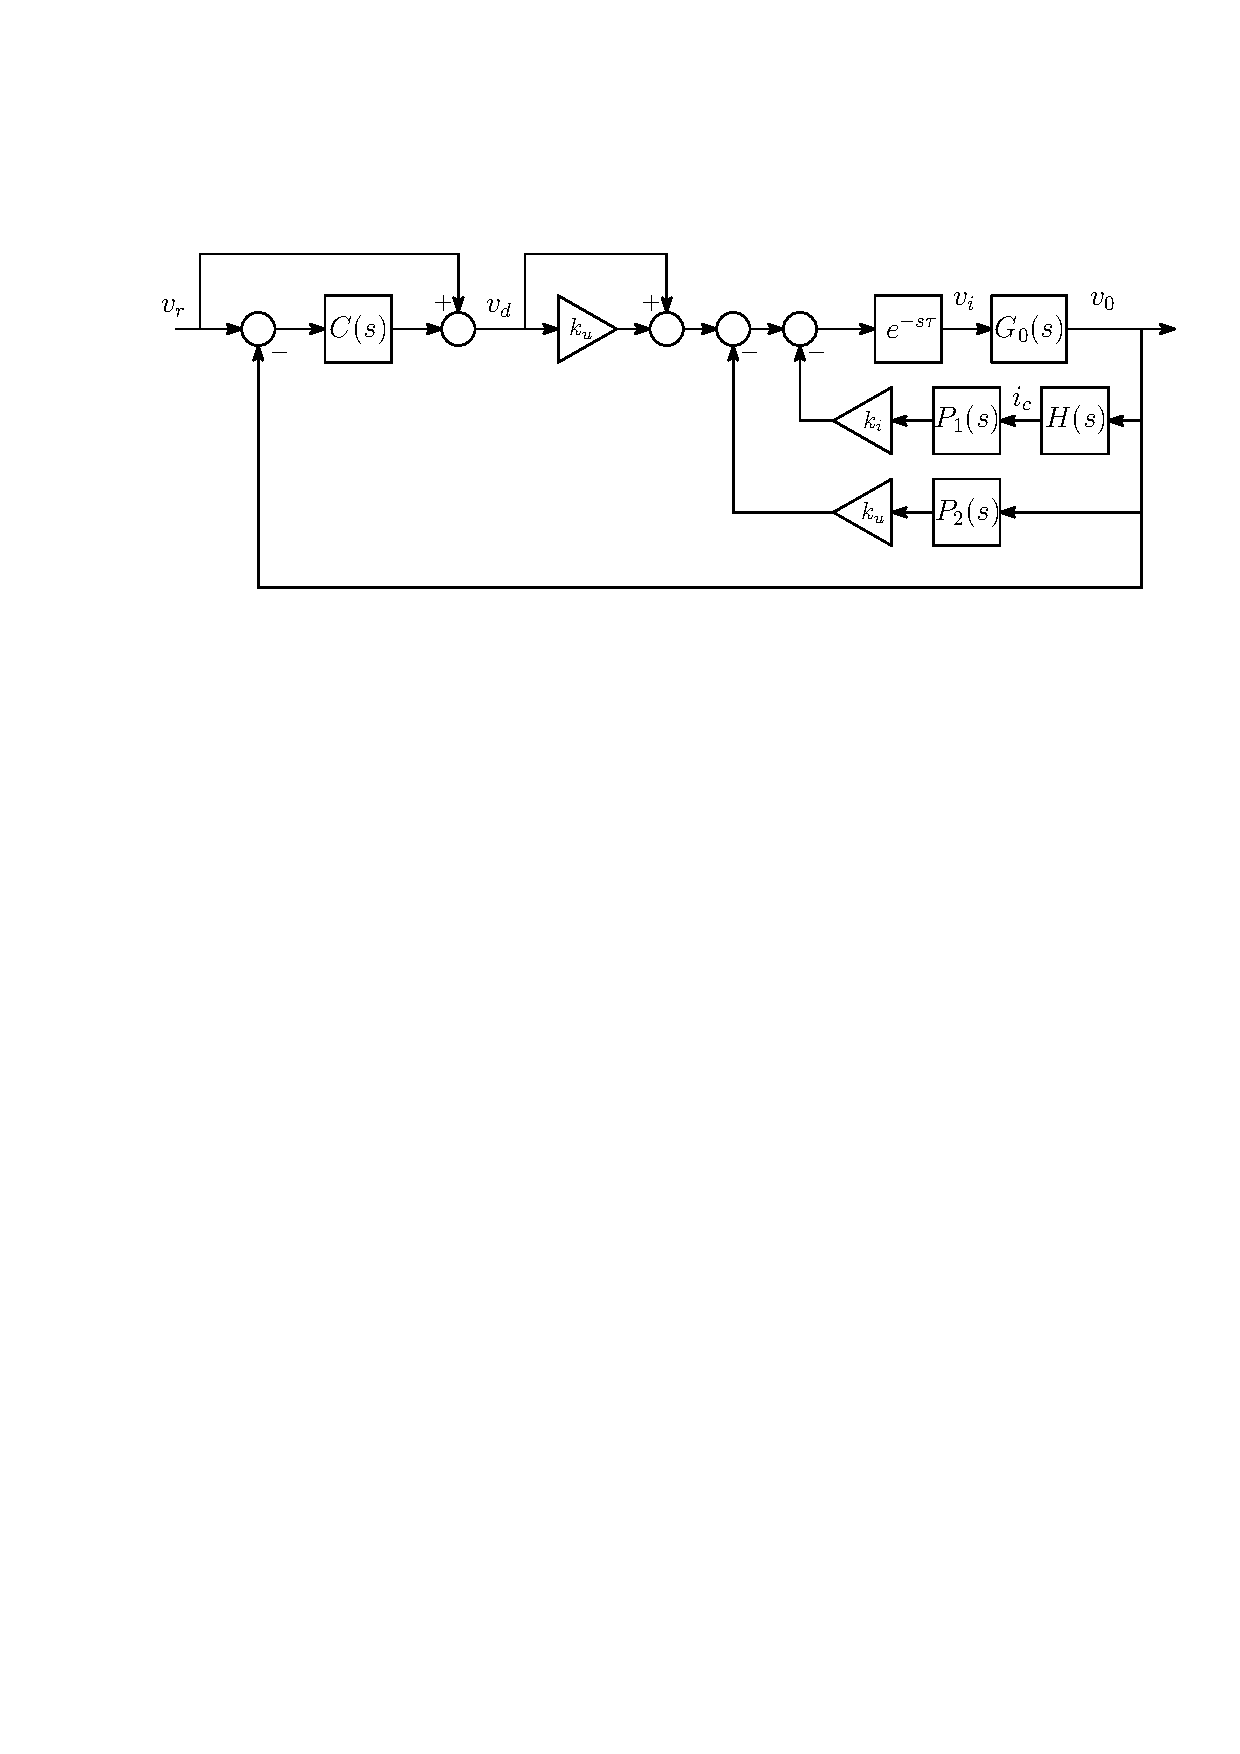
\includegraphics[width=\columnwidth]{../pics/damping_loop_full}
\caption{Interconnection of the power converter control system. }
\label{fig:damping_loop}
\end{figure}
$G_0(s)$ represents the TF from $v_i$ to $v_0$ in Fig.~\ref{fig:circuit}; $H(s)$ represents the TF from $v_0$ to $i_c$; $P_1(s)$ and $P_2(s)$ are sensors (i.e., low-pass filters); $k_i$ and $k_u$ are the control variable gains; $T_\alpha \: [s]$ is an actuation delay; and $C(s)$ is a PI controller (i.e., $C(s) = k_{p_1} + s^{-1}k_{p_2}$). From this framework, it can be observed that the inner feedback loops are reminiscent of a state-feedback control architecture while the system (as a whole) is a common unity feedback structure with feedforward action. For this application, note that $\{G_0,P_1,P_2 \} \in \mathscr{S}$ and $H \in \mathscr{P}$. The objective of this application is to design controllers such the TF from $v_d$ to $v_0$ and $v_r$ to $v_0$ both achieve the desired loop-shapes.

In order to simplify the system framework, let us define the following quantities:
\begin{equation} \label{eq:new_var}
\begin{aligned}
k_{m_1} &:= k_{p_1}(1+k_u) ;  &k_{m_2} &:= k_{p_2}(1+k_u)  \\
H_1(s,k) &:= k_iP_1(s)H(s);  &H_2(s,k) &:= k_uP_2(s) \\
G_d(s) &:= G_0(s)e^{-sT_\alpha}; &C_m(s,k) &:= k_{m_1}+s^{-1}k_{m_2}\\ 
\end{aligned}
\end{equation}
where $k \in \{k_i,k_u,k_{m_1},k_{m_2}\}$. Let the TF from $v_d$ to $v_0$ be denoted as $T^{\prime}(s,k)$ and the TF from $v_r$ to $v_0$ be denoted as $T(s,k)$.  Then these closed-loop TF's can easily be derived as follows:

\begin{align}
T^{\prime}(s,k) &= \frac{G_d(s)(1+k_u)}{1+G_d(s)[H_1(s,k)+H_2(s,k)]} \label{eq:Tclp}  \\ 
T(s,k) &= \frac{G_d(s)[1+k_u+C_m(s,k)]}{1+G_d(s)[H_1(s,k)+H_2(s,k)+C_m(s,k)]}  \label{eq:Tcl} 
\end{align}

For the remaining theoretical portions of this document, the loop-shaping technique will only be shown for $T(s,k)$, since the same procedures can also be applied to $T^{\prime}(s,k)$. Additionally, for notation purposes, the dependency in $s$ will be omitted and reiterated when deemed necessary. Additionally, all functions discussed hereafter will be FRF's with $s = j\omega$. For example, the denotation $T(k)$ represents $T(j\omega,k)$.



\section{Main Results}
\label{sec:main}
In this section, it will be demonstrated that the performance specification of the control problem will be achieved by formulating a convex optimization problem. The controllers will be synthesized by only considering the FRF of the system components.

\subsection{Convex Approximation}
The type of optimization problem that will be considered in the paper will have the following form:

\begin{equation} \label{eq:con_cav}
\begin{aligned}
& \underset{ x }{\text{minimize}}
& & \gamma  \\
& \text{subject to:} & & y(x)-z(x) < \gamma 
\end{aligned}
\end{equation}

where $y(x)$ and $z(x)$ are both convex functions of $x$ and $\{ \gamma \in \mathbb{R} : \gamma > 0\}$. This type of problem is convex-concave (due to the $-z(x)$ term); one solution to convexify this problem is to linearize $z(x)$ around an operating point $x_0$ and obtain the following optimization problem:

\begin{equation} \label{eq:con_lin}
\begin{aligned}
& \underset{ x }{\text{minimize}}
& & \gamma  \\
& \text{subject to:} & & y(x)-\bigl[ \nabla z(x_0) \bigr]^{\top} (x-x_0) < \gamma 
\end{aligned}
\end{equation}

 where $\nabla z(x_0)$ is the gradient of $z(x)$ evaluated at $x_0$. 
 
The control methodology in this paper is based on minimizing a control objective in the $\mathcal{H}_\infty$ or $\mathcal{H}_2$ sense. In subsequent sections, it will be shown that these performance constraints will have the following quadratic form:

\begin{equation} \label{eq:basic_ineq}
y^{\star}(x) \gamma^{-1} y(x) - z^{\star}(x)z(x) < 0 
\end{equation} 

where $y(x)$ and $z(x)$ are complex affine functions of the decision variable $x$ and $(\cdot)^{\star}$ denotes the complex conjugate of the argument. Let $f(x) = z^{\star}(x)z(x)$ with $z(x)$ defined as

$$z(x) = a_0 + a_1x_1 + a_2x_2 + ,\ldots , + a_nx_n$$

where $z:\mathbb{R}^n \rightarrow \mathbb{C}$ and $f:\mathbb{R}^n \rightarrow \mathbb{R}$. A first order Taylor series of $f(x)$ around an operating point $x_0$ can be formulated as follows:

\begin{equation} \label{eq:lin_fx}
f(x) \approx f(x_0) + D_f(x_0)[x-x_0]
\end{equation}

where
$$D_f(x_0) = \left[ \frac{\partial f(x)}{x_1}\Bigr|_{x=x_0}, \frac{\partial f(x)}{x_2}\Bigr|_{x=x_0},\ldots, \frac{\partial f(x)}{x_n}\Bigr|_{x=x_0}\right]$$

Without loss of generality, it can be shown that the left-hand side of (\ref{eq:lin_fx}) will always be greater than or equal to the right-hand side, i.e.,

\begin{equation} \label{eq:lin_inequality}
z^{\star}(x)z(x) \geq z^{\star}(x)z_0 + z(x)z_0^{\star} - z_0^{\star}z_0
\end{equation} 

where $z_0 = z(x_0)$. The condition in (\ref{eq:lin_inequality}) can easily be established by realizing the following inequality:

\begin{equation}
[z(x)-z_0]^{\star}[z(x)-z_0] \geq 0
\end{equation}

With this linearization, a sufficient condition for the inequality in (\ref{eq:basic_ineq}) can be developed as follows:

\begin{equation}
y^{\star}(x) \gamma^{-1} y(x) - [z^{\star}(x)z_0 + z(x)z_0^{\star} - z_0^{\star}z_0]< 0 
\end{equation}

By using the Shur Complement Lemma \cite{BEN09}, the above condition can be expressed in terms of a Linear-Matrix-Inequality (LMI):

\begin{equation} \label{eq:LMI_1}
\begin{bmatrix}
z^{\star}(x)z_0 + z(x)z_0^{\star} - z_0^{\star}z_0 & \phantom{xx} y^{\star}(x) \\
y(x) & \phantom{xx} \gamma
\end{bmatrix}
\succ 0
\end{equation}

This type of formulation will be used in section \ref{sec:loop_shape} in order to construct a loop-shaping constraint on the closed-loop FRF.

\subsection{Control Performance}
Since the control methods discussed in this paper are based on the $\mathcal{H}_\infty$ criterion, it is appropriate to first define this criterion in the context of this work. A typical control objective is to design a controller such that the following constraint is satisfied:
\begin{equation} \label{eq:WS_lt1}
\| W_q \mathcal{S}_q\| < 1
\end{equation}
where $\mathcal{S}_q$ is the $q$-th sensitivity function of interest, and $W_q$ is a stable weighting function such that $\| W_q \mathcal{S}_q\|$ is bounded. The norm considered in (\ref{eq:WS_lt1}) can be either the 2- or infinity-norm. 

For SISO systems, and for a stable system $X(s)$, the 2- and infinity-norms are defined as follows:
\begin{align*}
\| X\|_2^2 & := \frac{1}{2\pi} \int_{- \infty}^\infty |X(j\omega)|^2 d\omega \\
\| X\|_\infty & :=  \sup_{\omega} |X(j\omega)|
\end{align*}
It is imperative to note that the boundedness of spectral norm $X$ does not guarantee the stability of $X$. 

A loop-shaping criterion can also be considered as a form of control performance. If $T$ is the closed-loop FRF and $T_d$ is the desired FRF, then one can consider minimizing $(T-T_d)$ in either the 2- or infinity-norm sense in order to shape $T$.  The next section will discuss how an optimization problem can be formulated for this type of control methodology.

\subsection{Loop-Shaping Design}
\label{sec:loop_shape}
As asserted in section \ref{sec:system}, the objective of this control problem is to shape the FRF of $T(k)$. Suppose that a desired loop-shape is specified as $T_d$; the objective is to design gains in $k$ such that the closed-loop system $T(k)$ coincides with $T_d$ in the $\mathcal{H}_\infty$ or $\mathcal{H}_2$ sense. In the $\mathcal{H}_\infty$ sense, the objective is to minimize $ \|T(k) - T_d \|_\infty$; an equivalent representation of this objective is to minimize $\gamma$ such that $ \|T(k) - T_d \|_\infty < \gamma$. This criterion is satisfied if the the following optimization problem is considered:
 
 \begin{equation} \label{eq:min_loopshape}
\begin{aligned}
& \underset{ k \in \mathbb{R}}{\text{minimize}}
& & \gamma  \\
& \text{subject to:} & & \bigl[T(k)-T_d\bigr]^{\star}\bigl[T(k)-T_d\bigr] < \gamma
\end{aligned}
\end{equation}
for all $\omega \in \Omega$. It can be observed that the constraint in (\ref{eq:min_loopshape}) is not convex. Let $z(k) = 1+G_d[H_1(k)+H_2(k)+C_m(k)]$ and $N(k) = G_d[1+k_u+C_m(k)]$; then the above constraint can be written as:

\begin{equation}
\bigl[N(k)-z(k)T_d \bigr]^{\star}\gamma^{-1} \bigl[N(k)-z(k)T_d \bigr] - z^{\star}(k)z(k)<0
\end{equation} 

Note that this constraint has the exact form as in (\ref{eq:basic_ineq}); therefore, the convex constraint in (\ref{eq:LMI_1}) can be utilized to construct the loop-shaping optimization problem as follows:

\begin{equation} \label{eq:loop_shape_LMI_inf}
\begin{aligned}
& \underset{ k \in \mathbb{R}}{\text{minimize}} \hspace{0.5cm} \gamma  \\
& \text{subject to:} \\
&
\begin{bmatrix}
z^{\star}(k)z_0 + z_0^{\star}z(k) - z_0^{\star}z_0 & \phantom{xx}[N(k)-z(k)T_d]^{\star} \\ 
N(k)-z(k)T_d & \phantom{xx}\gamma
\end{bmatrix} \succ 0
\end{aligned}
\end{equation}
for all $\omega \in \Omega$, where $z_0 = 1+G_d[H_1(k_0) + H_2(k_0)+C_m(k_0)]$ and $k_0 \in \{k_{i,0},k_{u,0},k_{m_1,0},k_{m_2,0}  \}$ are the initializing gains. In a similar manner, the following convex optimization problem can be considered for minimizing  $ \|T(k)- T_d \|_2^2$, as follows:

\begin{equation} \label{eq:loop_shape_LMI_2}
\begin{aligned}
& \underset{ k \in \mathbb{R}}{\text{minimize}} \hspace{0.5cm} \int_0^\infty \gamma(\omega) d\omega  \\
& \text{subject to:} \\
&
\begin{bmatrix}
z^{\star}(k)z_0 + z_0^{\star}z(k) - z_0^{\star}z_0 & \phantom{xx}[N(k)-z(k)T_d]^{\star} \\ 
N(k)-z(k)T_d & \phantom{xx}\gamma(\omega)
\end{bmatrix} \succ 0
\end{aligned}
\end{equation}
for all $\omega \in \Omega$. For this $\mathcal{H}_2$ problem, note that $\gamma$ is now a function of $\omega$ (which contrasts with the optimization problem in the $\mathcal{H}_\infty$ sense). 

\iffalse
If it is desired to minimize the $\mathcal{H}_\infty$ norm of a weighted sensitivity function, one can easily formulate an optimization problem to minimize $ \|W_q \mathcal{S}_q(k)\|_\infty$, i.e.,
 \begin{equation} \label{eq:min_weighted_norm}
\begin{aligned}
& \underset{ k \in \mathbb{R}}{\text{minimize}}
& & \gamma  \\
& \text{subject to:} & & \bigl[W_q \mathcal{S}_q(k)\bigr]^{\star}\bigl[W_q \mathcal{S}_q(k)\bigr] < \gamma
\end{aligned}
\end{equation}
Then, as was shown in (\ref{eq:min_loopshape})-(\ref{eq:loop_shape_LMI_inf}) for the loop-shaping problem, a corresponding LMI can be derived for the $\infty$-norm of the weighted sensitivity function. In a similar manner, the convex optimization problem can be derived for minimizing the 2-norm of the weighted sensitivity function (i.e., minimize $ \|W_q \mathcal{S}_q(k)\|_2^2$). 
\fi

{\bf Remark:} 
\textit{Note that the choice of the initializing gains in $k_0$ may affect the stability of the closed-loop system (for either the optimization problems concerning the $\mathcal{H}_\infty$ or $\mathcal{H}_2$ norms). The next section will discuss how to select these gains in order to ensure stability. \\ 
Additionally, note that these optimization problems are considering the gains for $C_m(k)$; however, once an optimal solution is obtained for the gains in $k$, then the definitions in (\ref{eq:new_var}) can be used to revert back to the original gains (i.e., $k_{p_1}$ and $k_{p_2}$.)}


\subsection{Stability Analysis}
The loop-shaping constraints developed in the previous section do not guarantee the closed-loop stability of the closed-loop system. Setting a desired FRF to shape a closed-loop FRF is analogous to bounding the closed-loop FRF; it can be shown that unstable systems can still possess bounded FRF's. 

The initializing gains in $k_0$ play an important role in guaranteeing the stability of the closed-loop system. By using the Nyquist criterion for continuous-time systems, the stability of the closed-loop system can be ensured if certain conditions are met for these initializing gains. Let us first recall the Nyquist stability criterion with the following Lemma:
\begin{lemma}
A closed-loop system with a plant $G(s)$ and a controller $C(s)$ in a unity-feedback structure is stable if and only if the Nyquist plot of $1+G(s)C(s)$
\begin{itemize}
\item makes $n_G + n_C$ counterclockwise encirclements of the origin, where $n_G$ and $n_C$ are the number of right-half-plane (RHP) poles of $G(s)$ and $C(s)$, respectively
\item does not pass through the origin
\end{itemize}
\end{lemma}
Note that in this Nyquist stability criterion, the term $GC$ refers to the open-loop system. In this paper, it is assumed that the Nyquist contour has some small detours around the poles of $G$ and $C$ on the imaginary axis.

The following properties will be needed in order to properly analyze the stability conditions of the system:
\begin{definition}
Let wno$\{ A(s)\}$ refer to the winding number; in the counterclockwise sense, wno$\{ A(s)\}$ represents the image of $A(s)$ around the origin when $s$ traverses the Nyquist contour (with small detours around the poles of $A(s)$ on the imaginary axis). Then the following properties hold:
\begin{align}
\text{wno}\bigl\{ A_1(s)A_2(s) \bigr\} &= \text{wno}\bigl\{ A_1(s) \bigr\} + \text{wno}\bigl\{ A_2(s) \bigr\}  \label{eq:wno_add}\\ 
\text{wno}\bigl\{ A(s)\bigr\} &= -\text{wno}\bigl\{ A^{\star}(s)\bigr\} \label{eq:wno_conj} \\ 
\text{wno}\bigl\{ A(s)\bigr\} &= -\text{wno}\bigl\{ A^{-1}(s)\bigr\} \label{eq:wno_inv}
\end{align}
\end{definition}

The open-loop FRF from the system in Fig.~\ref{fig:damping_loop} is given as $$L(k) = G_d[H_1(k)+H_2(k)+C_m(k)].$$ Let $F(k) = H_1(k)+H_2(k)+C_m(k)$ such that $L(k) = G_dF(k)$; by the Nyquist stability criterion, the closed-loop system is stable if and only if $1+G_dF$ makes $n_{G_d}+n_F$ counter-clockwise encirclements of the origin (where $n_{G_d}$ and $n_F$ are, respectively, the number of RHP poles of $G_d$ and $F$). The Nyquist plot of $1+G_dF$ must also not pass through the origin.

\begin{theorem} \label{Thm1}
Suppose that $k_i$, $k_u$, $k_{m_1}$, and $k_{m_2}$ are feasible solutions to the following constraint:
\begin{equation} \label{eq:theorem1_cond}
\begin{split}
z^{\star}(k)z_0+z_0^{\star}z(k) > 0 \\
\forall \omega \in \Omega
\end{split}
\end{equation}
where 
\begin{align*}
z(k) &= 1+G_d[H_1(k)+H_2(k)+C_m(k)] \\
z_0 &= 1+G_d[H_1(k_0)+H_2(k_0)+C_m(k_0)]
\end{align*}
with $\{G_d,H_1,H_2\} \in \mathscr{S}$. Then the closed-loop system $T$ is stable if the parameters in the set $k_0$ are stabilizing initial gains.
\end{theorem}

\textit{Proof:}
The proof is based on the Nyquist stability criterion and the properties of the winding number. The winding number of $z^{\star}(k)z_0$ is given as follows:
\begin{equation} \label{eq:winding_proof}
\begin{aligned}
{\mbox{wno}} \{ z^{\star}(k)z_0\} &= {\mbox{wno}} \{ z^{\star}\} + {\mbox{wno}} \{ z_0\} \\
&= -{\mbox{wno}} \{ 1+G_dF(k)\} \\
&\phantom{=} + {\mbox{wno}} \{ 1+G_dF(k_0)\} \\
\end{aligned}
\end{equation}
where $F(k_0) = H_1(k_0) + H_2(k_0) + C_m(k_0)$. Note that $F(k)$ is strictly proper and $G_dF(k)$ is strictly proper; therefore, the winding number of $z^{\star}(k)z_0$ can be evaluated over $\Omega$ instead of the $D$-contour. Additionally, the constraint in (\ref{eq:theorem1_cond}) implies that $\Re\{ z^{\star}(k)z_0\} > 0$ (where $\Re\{ \cdot \}$ indicates the real part of the argument), which signifies that the Nyquist plot of $z^{\star}(k)z_0$ will not pass through or encircle the origin. Therefore, $\mbox{wno} \{ z^{\star}(k)z_0\} = 0$; from (\ref{eq:winding_proof}), the following condition can then be realized:
\begin{equation} \label{eq:winding_proof3}
\mbox{wno} \{ 1+G_dF(k)\} = {\mbox{wno}} \{ 1+G_dF(k_0)\}
\end{equation}
The condition in (\ref{eq:winding_proof3}) implies that if the initializing controllers $k_0$ are stabilizing (i.e., the open-loop system $G_dF(k_0)$ meets the Nyquist stability criterion), then the closed-loop system will be stable.
{\hfill \ensuremath{\blacksquare}}

\subsection{Initializing Controller}
For the given structure in Figure.~\ref{fig:damping_loop} , it remains to show how to select the initial stabilizing controllers in order to guarantee the stability of the closed-loop system. From the control structure of the power converter control system, it can be observed that if all the gains in Figure.~\ref{fig:damping_loop} are set to zero, then the system will be in open-loop. However, since $G_d \in \mathscr{S}$, then selecting $k_0 = 0$ will guarentee the stability of the closed-loop system. 

If the initializing controllers are selected such that the performance with these controllers is far from the desired performance, then it is possible that either the optimization problem yields no feasible solution, or that the solver runs into numerical problems (which leads to infeasible solutions). One method to resolve this problem is to apply relaxation techniques where a relaxed optimization problem is solved; the solution to the relaxed problem is then used as the initializing controllers for the non-relaxed problem. 


\subsection{Convex Optimization via Semi-Definite Programming}
All of the optimization problems considered in section \ref{sec:loop_shape} are known as semi-infinite programming (SIP) problems since there are a finite number of optimization variables $k$ and an infinite number of constraints with respect to $\omega$. To solve any of these problems, the optimization algorithm can be converted to a semi-definite programming (SDP) problem. In this manner, a predefined frequency grid can be implemented in order to solve a finite number of constraints. In other words, for a finite number of frequency points $n$ selected in $\omega \in [0,\infty)$, then $n$ constraints must be satisfied. This frequency grid can be predefined in a variety of manners (see \cite{SVBB11}, \cite{GKL10b}, \cite{FR05}). 

\section{Case Study}
\label{sec:case}
The focus of this case study will be on the SATURN power converter, which incorporates the control methodology shown in Figure.~\ref{fig:damping_loop} and uses the filter shown in Figure.~\ref{fig:circuit}. The SATURN converter is used in the Large Hardron Collider, in injector machines, in experimental areas to power warm magnets, and for DC or pulsed applications. In this power converter, a $18\:kV/50\:Hz$ transformer is used with a diode rectifier and a DC-Link filter for the AC/DC conversion. An IGBT bridge (4 quadrant operation) is then used for a DC/DC conversion, and the output of this bridge is then fed into the filter (i.e, $v_i$ in Fig.~\ref{fig:circuit}). For this application, two identical modules are assembled in series (which doubles the output voltage) where the equivalent switching frequency of this bridge is $5 \: kHz$. A schematic of the SATURN modules are shown in Fig.~ \ref{fig:schematic}. A complete assembly of the SATURN power converter is shown in Fig.~\ref{fig:saturn_pc} while the load (i.e., the $RL$ circuit representing the magnet) is shown in Fig.~\ref{fig:load}.

\begin{figure}
\centering
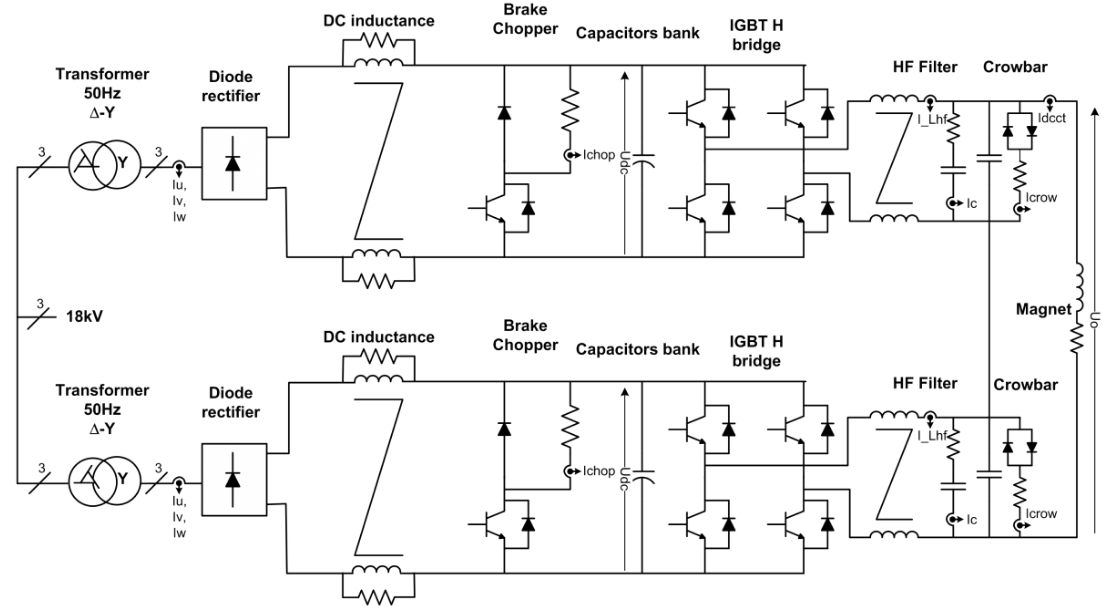
\includegraphics[width=\columnwidth]{../pics/schematic}
\caption{Schematic of the SATURN modules set in series.}
\label{fig:schematic}
\end{figure} 

\begin{figure}
\centering
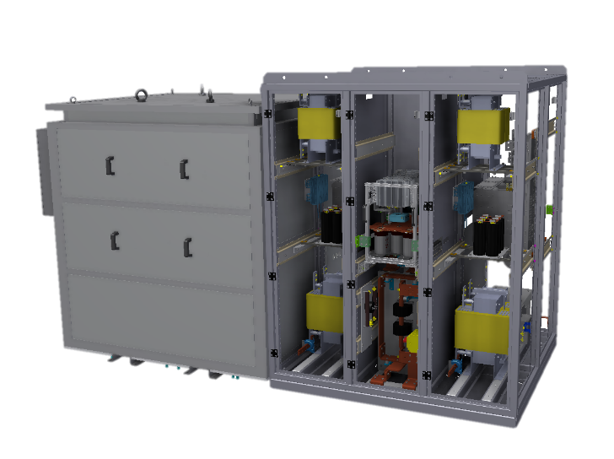
\includegraphics[width=\columnwidth]{../pics/Saturn_1}
\caption{SATURN power converter used for various applications at CERN.}
\label{fig:saturn_pc}
\end{figure} 

\begin{figure}
\centering
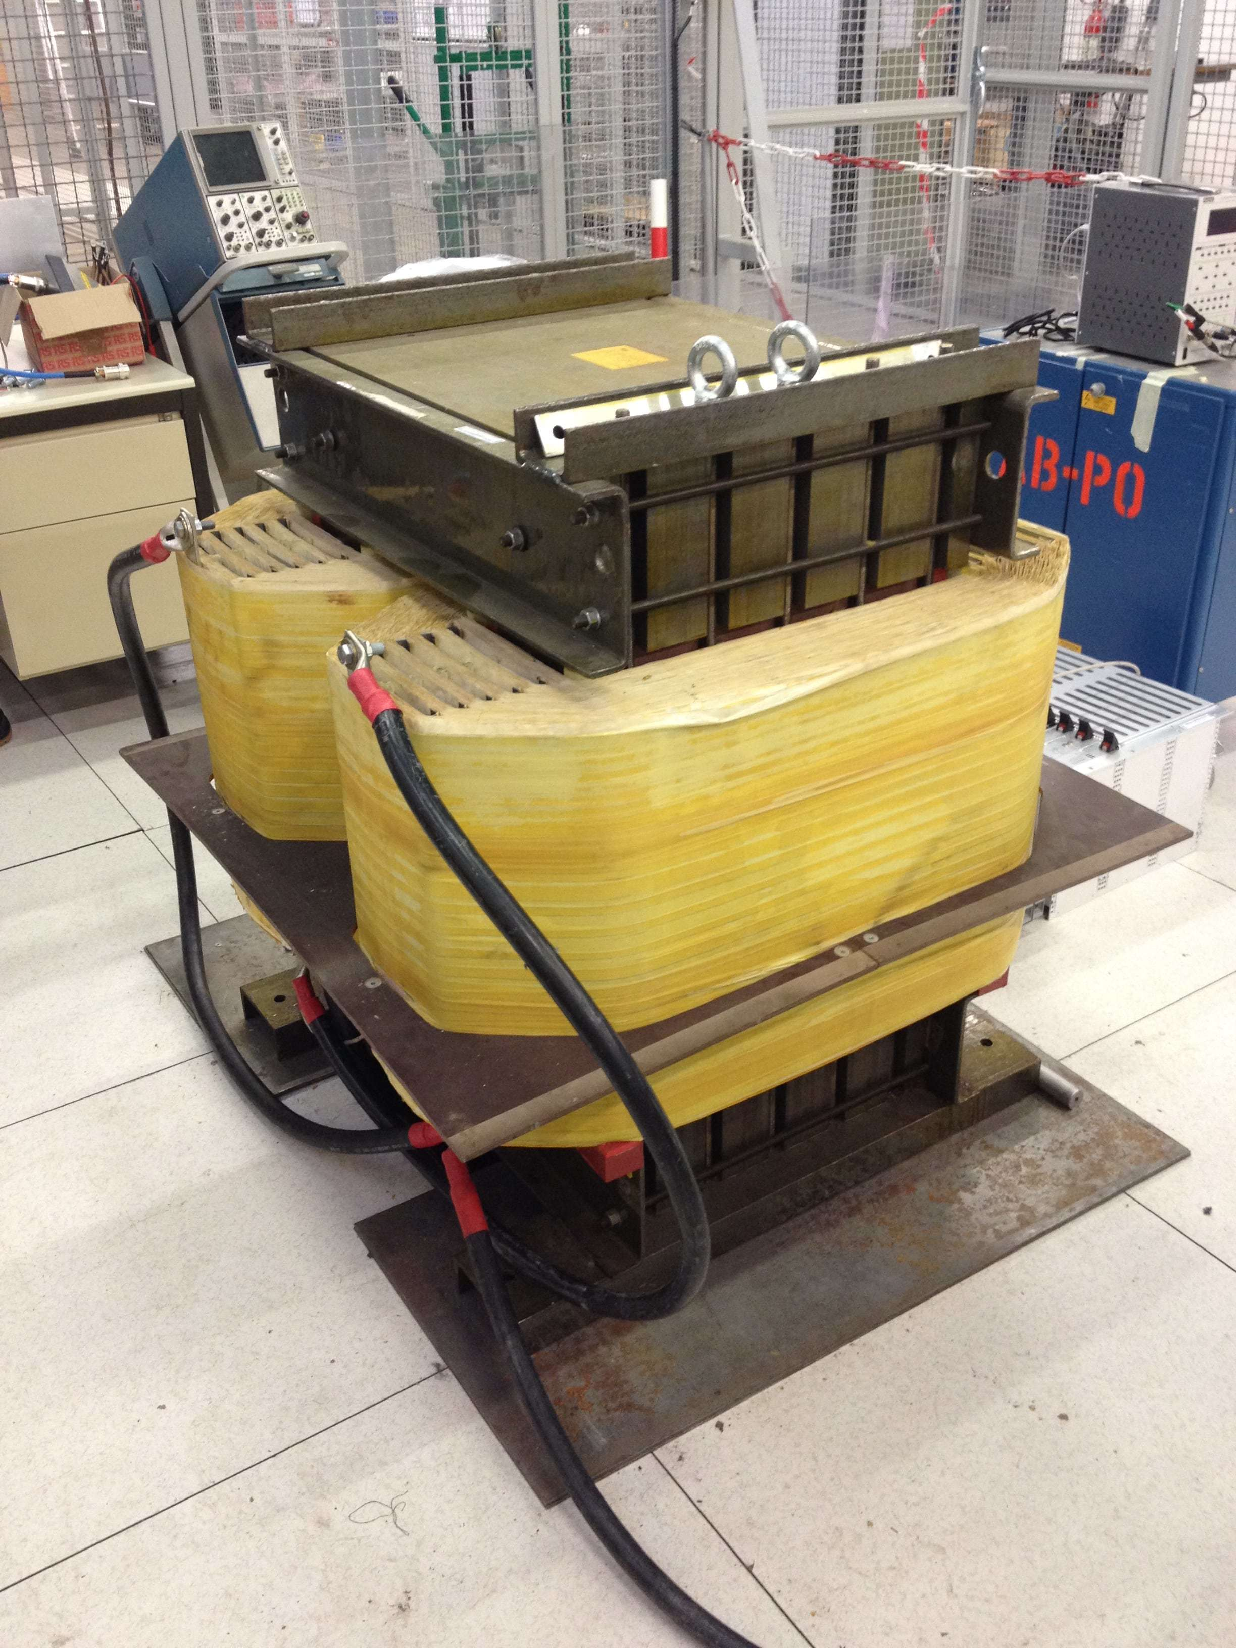
\includegraphics[width=\columnwidth, height=8cm]{../pics/load}
\caption{The SATURN load which is used to mimic the dynamics of the magnet.}
\label{fig:load}
\end{figure} 

\subsection{Frequency Response Measurement}
Since the proposed method uses a data-driven methodology with frequency-domain data, the frequency response of each subsystem within the power converter control system must be obtained. In other words, we must obtain the frequency responses of $G_d$, $H$, $P_1$, and $P_2$. The signals that are accessible for the measurements are the inputs to the capacitor banks ($U_{dc}$ in Fig.~\ref{fig:schematic}), and the outputs of the sensors $P_1$ and $P_2$. Therefore, when all of the controller gains are set to zero, we are able to obtain the frequency responses of $G_dHP_1$ and $G_dP_2$. However, note that $G_d$ appears independently of $P_2$ in (\ref{eq:Tclp}) and (\ref{eq:Tcl}); since $P_1$ and $P_2$ are sensors with very high bandwidths relative to $G_d$ (approximately $10 \: kHz$), then $G_d \approx G_dP_2$  at frequencies less than $1 \: kHz$. 

The frequency response of the subsystems were obtained with a transfer function analyzer (Powertek GP102) which implements a sine-sweep method that recovers the gain and phase of a system at discrete frequency points. The appropriate scaling factors were taken into account for the measurements (due to the series connection of the SATURN modules) in order to coincide with the structure used in Fig.~\ref{fig:damping_loop}. The frequency responses of $G_dP_2$ and $G_dHP_1$ are shown in Fig.~\ref{fig:G} and Fig.~\ref{fig:GHP1}, respectively.

\begin{figure}
\centering
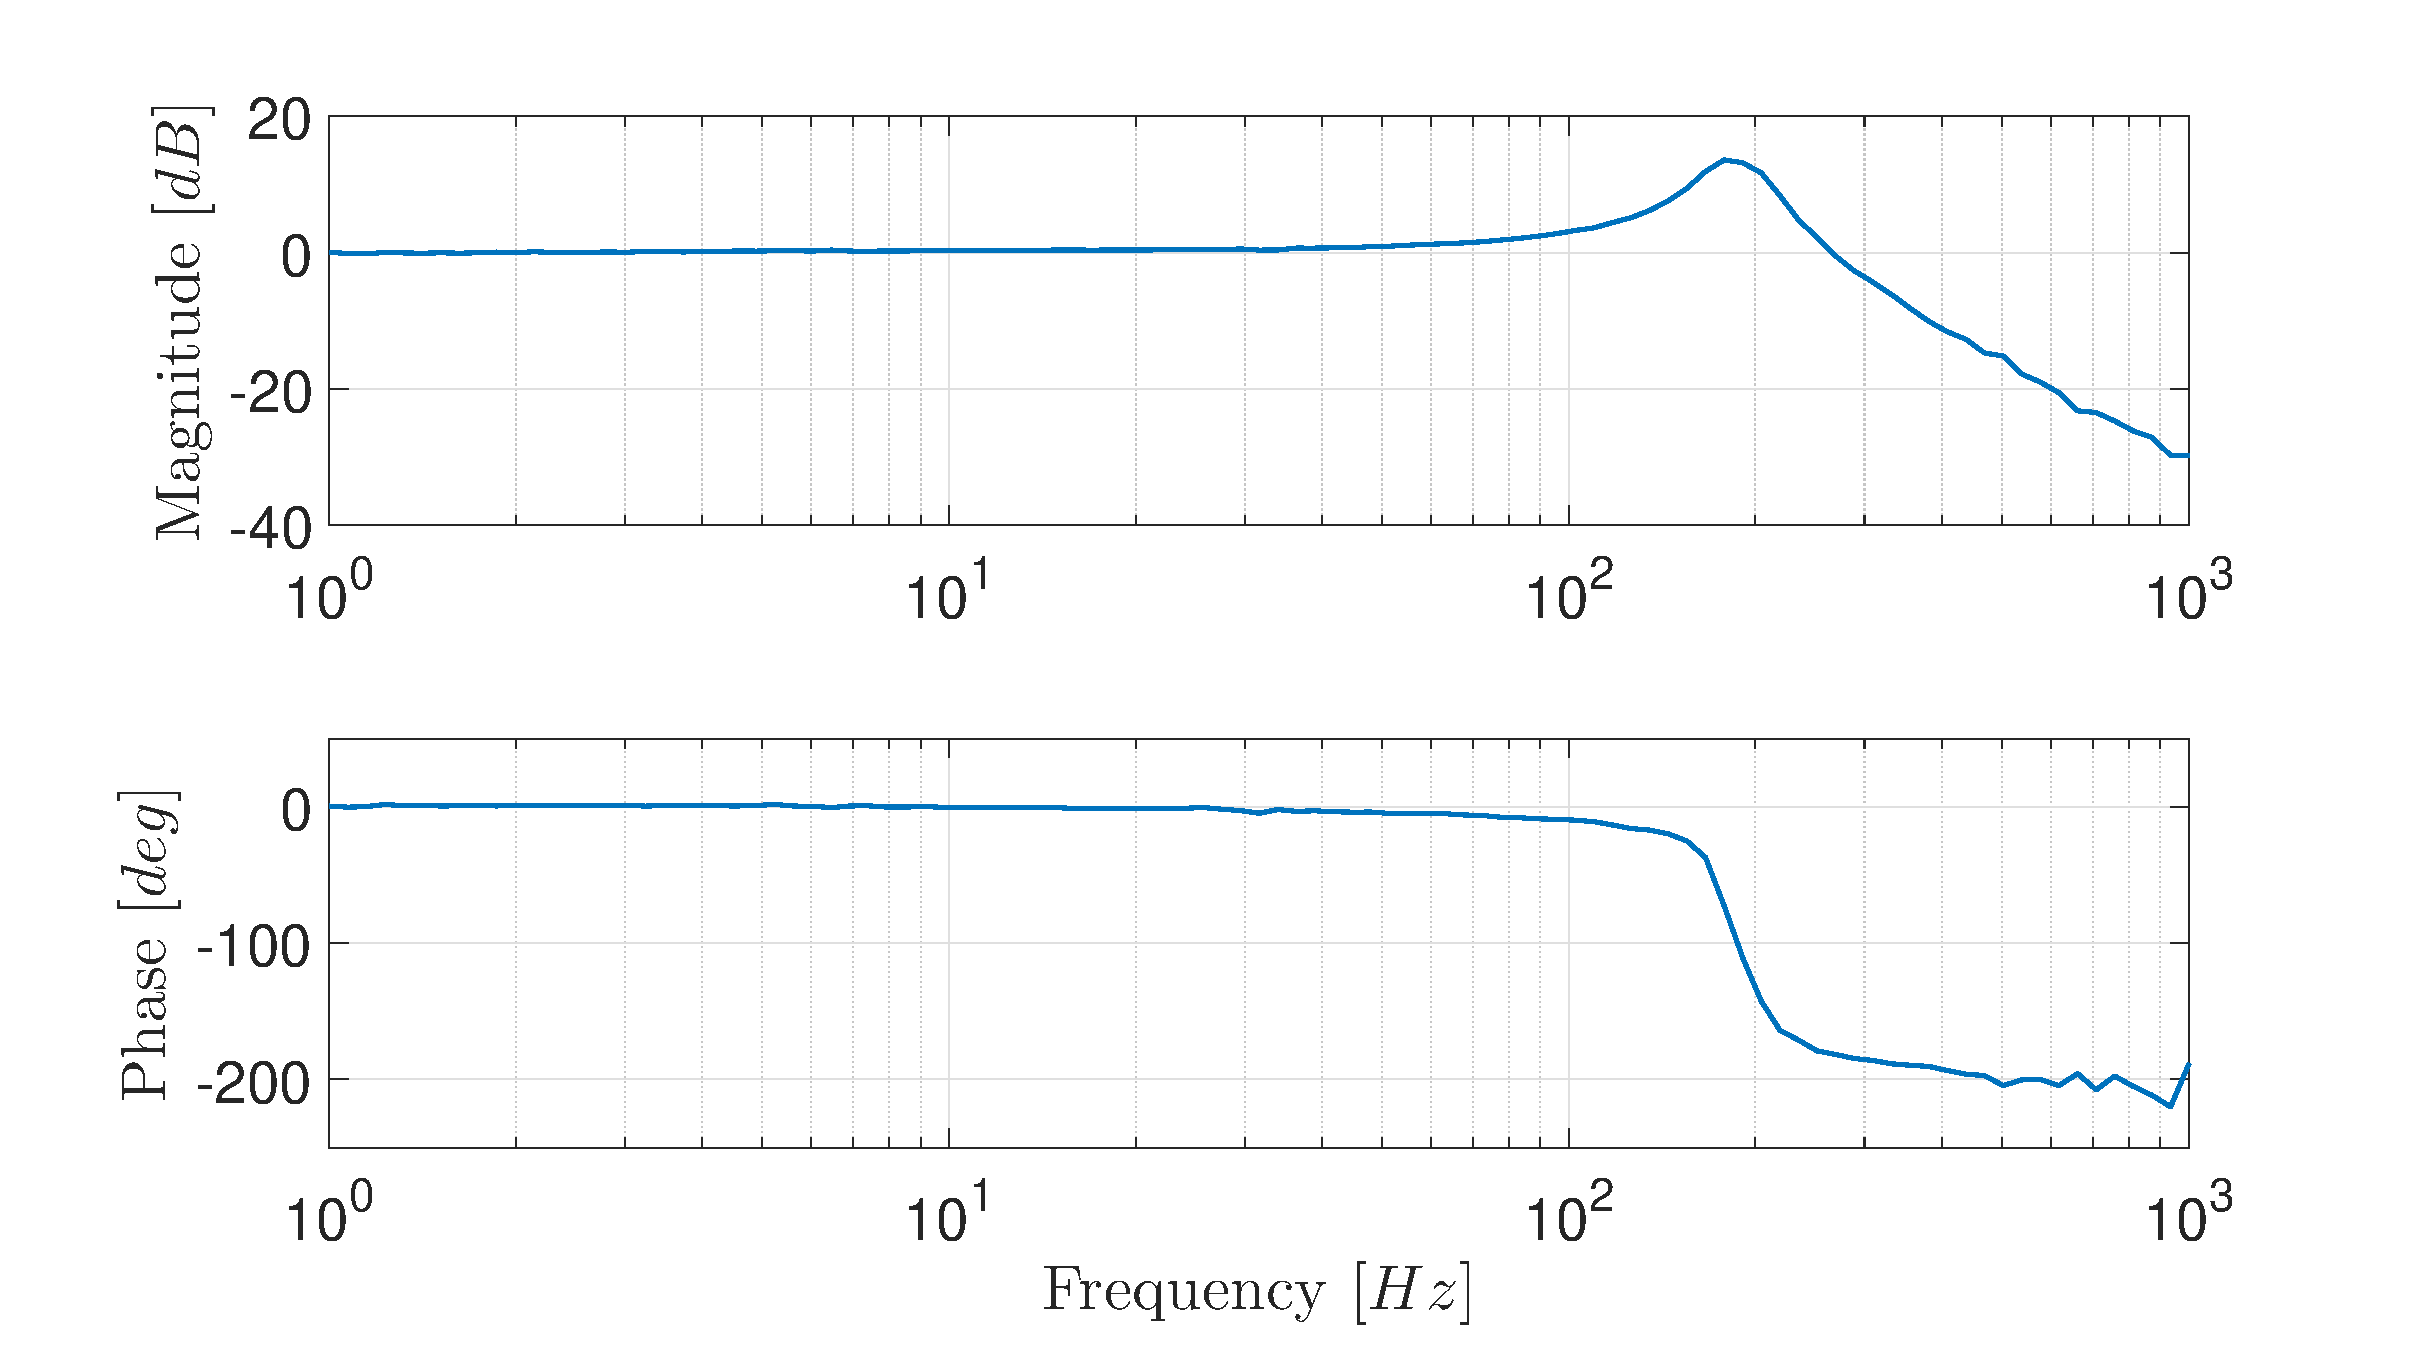
\includegraphics[width=\columnwidth]{../pics/G.eps}
\caption{Frequency response measurement from the input of the capacitor banks to the output of sensor $P_2$ (with all controller gains set to zero).}
\label{fig:G}
\end{figure} 

\begin{figure}
\centering
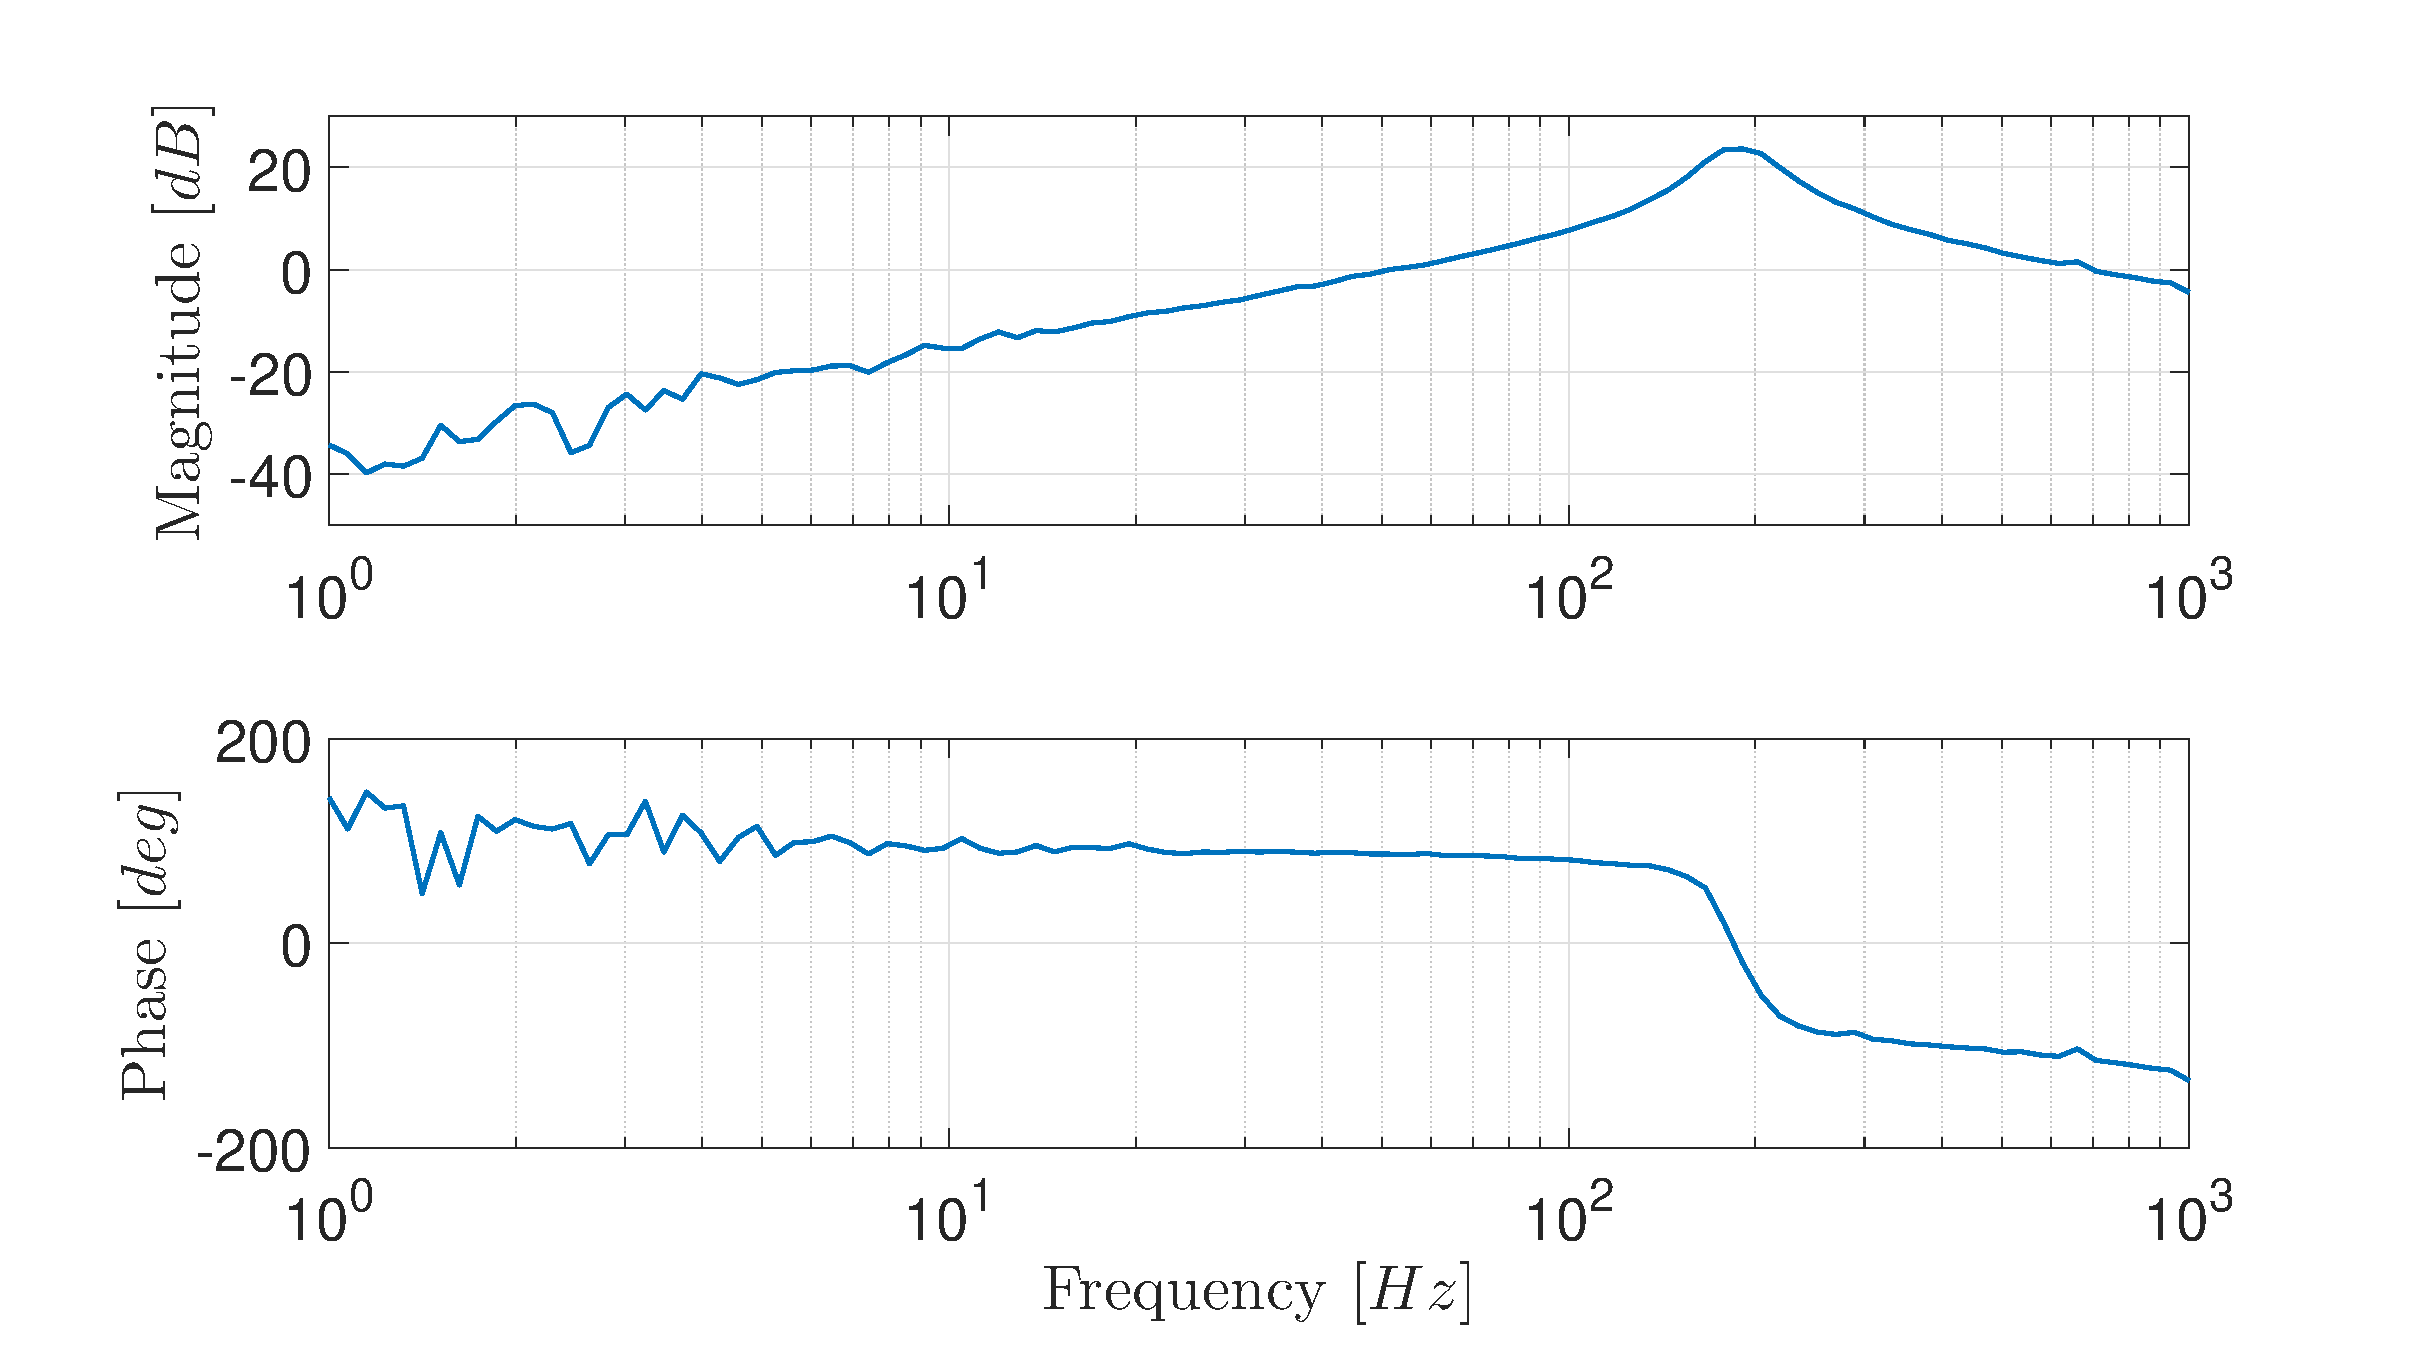
\includegraphics[width=\columnwidth]{../pics/GHP1.eps}
\caption{Frequency response measurement from the input of the capacitor banks to the output of sensor $P_1$ (with all controller gains set to zero).}
\label{fig:GHP1}
\end{figure} 

\subsection{Controller Synthesis}
For this application, it was desired to shape $T^{\prime}(k)$ and $T(k)$ such that a bandwidth of $300 \: Hz$ and $500 \: Hz$ is attained, respectively (where both achieve a damping of $\zeta = 0.8$). Note that in both of these TF's, a pure delay appears in the numerator; therefore, the performance of the loop-shape algorithm can be improved by specifying a desired loop-shape $T_d = T_d^*e^{-sT_\alpha}$ where $T_d^*$ was selected as a standard second order process, i.e.,
\begin{equation}
T_d^*(s) = \frac{\omega_d^2}{s^2 + 2\zeta \omega_d s + \omega_d^2}
\end{equation}
where $\zeta$ is the damping factor and
\begin{equation*}
\omega_d = \frac{2 \pi f_d}{\sqrt{1-2\zeta^2 + \sqrt{2-4\zeta^2 + 4\zeta^4}}}
\end{equation*}
where $f_d$ is the desired closed-loop bandwidth. In other words, $T_d$ is simply a delayed version of the second order process.

Although the delay in $G_d$ was captured in the frequency response measurement, it is known that there also exists an additional measurement delay $T_\beta$ that was not captured in the identification experiment. This delay occurs after digitization of the analog signals at the outputs of $P_1$ and $P_2$. The value of the delay is uncertain and is known to be in the range of $T_\beta \in [0,30]\mu s$. Therefore, a multi-model design can be considered where the additional delay can be gridded in this range and incorporated into the closed-loop TF's. The grid was established in intervals of $5 \: \mu s$ (i.e., $T_{\beta_i} = [0,5,\ldots30] \mu s$, $i = 1,\ldots,7$).  

In the $\mathcal{H}_{\infty}$ sense, the optimization problem to consider for this case study is as follows:
 \begin{equation} \label{eq:case_study_opt}
\begin{aligned}
& \underset{ k \in \mathbb{R}}{\text{minimize}}
& & \gamma  \\
& \text{subject to:} & & \|T_i(k)-T_d\|_{\infty}< \gamma \\
& &  &\|T_i^{\prime}(k)-T_d^{\prime}\|_{\infty}< \gamma \\ 
& & & i = 1,\ldots,7
\end{aligned}
\end{equation}
where $T_i(k)$ and $T_i^{\prime}(k)$ are the closed-loop TF's that incorporate the additional $i$-th delay in $T_{\beta_i}$; $T_d$ is the desired closed-loop TF for loop-shaping $T(k)$ (with a desired bandwidth of $f_d = 500 \: Hz$ and damping $\zeta = 0.8$); $T_d^{\prime}$ is the desired closed-loop TF for loop-shaping $T^{\prime}(k)$ (with a desired bandwidth of $f_d^{\prime} = 300 \: Hz$ and damping $\zeta^{\prime} = \zeta$). A similar optimization problem can be considered for minimizing the $\mathcal{H}_2$ norm of the process. This optimization problem can be transformed to the convex problem by implementing the methods outlined in section \ref{sec:loop_shape}. 
\subsection{Experimental Results}
The constraints in the optimization problem in (\ref{eq:case_study_opt}) were first converted to LMI constraints; the problem was then converted to an SDP problem (since the transfer function analyzer provides the gain and phase at discrete frequency points). For solving the $\mathcal{H}_2$ problem in SDP form, the objective function in (\ref{eq:loop_shape_LMI_2}) must be discretized where $\int \gamma(\omega) d\omega \rightarrow \sum_i \gamma(\omega_i)$.

For comparative purposes, controllers were designed by considering the model of the process. There is uncertainty associated with the delay $T_\alpha$; the range of this uncertainty is $T_\alpha \in [0,200]\mu s$. Therefore, for the model-based design, the problem in (\ref{eq:case_study_opt}) was solved by gridding in both $T_\alpha$ and $T_\beta$.

Fig.~\ref{fig:d_loop} shows the closed-loop frequency response of $|T^{\prime}(j\omega)|$ while Fig.~\ref{fig:v_loop} shows the closed-loop frequency response of $|T(j\omega)|$ for the solutions obtained by minimizing both the $\mathcal{H}_{\infty}$ and $\mathcal{H}_2$ norms of the process. From these figures, it can be observed that that model-based design produces the worst performance while the data-driven based design achieves the desired performance for both TF's. The performance achieved by the data-driven method (in both the $\mathcal{H}_{\infty}$ and $\mathcal{H}_2$ minimization cases) are comparable. 
\begin{figure}
\centering
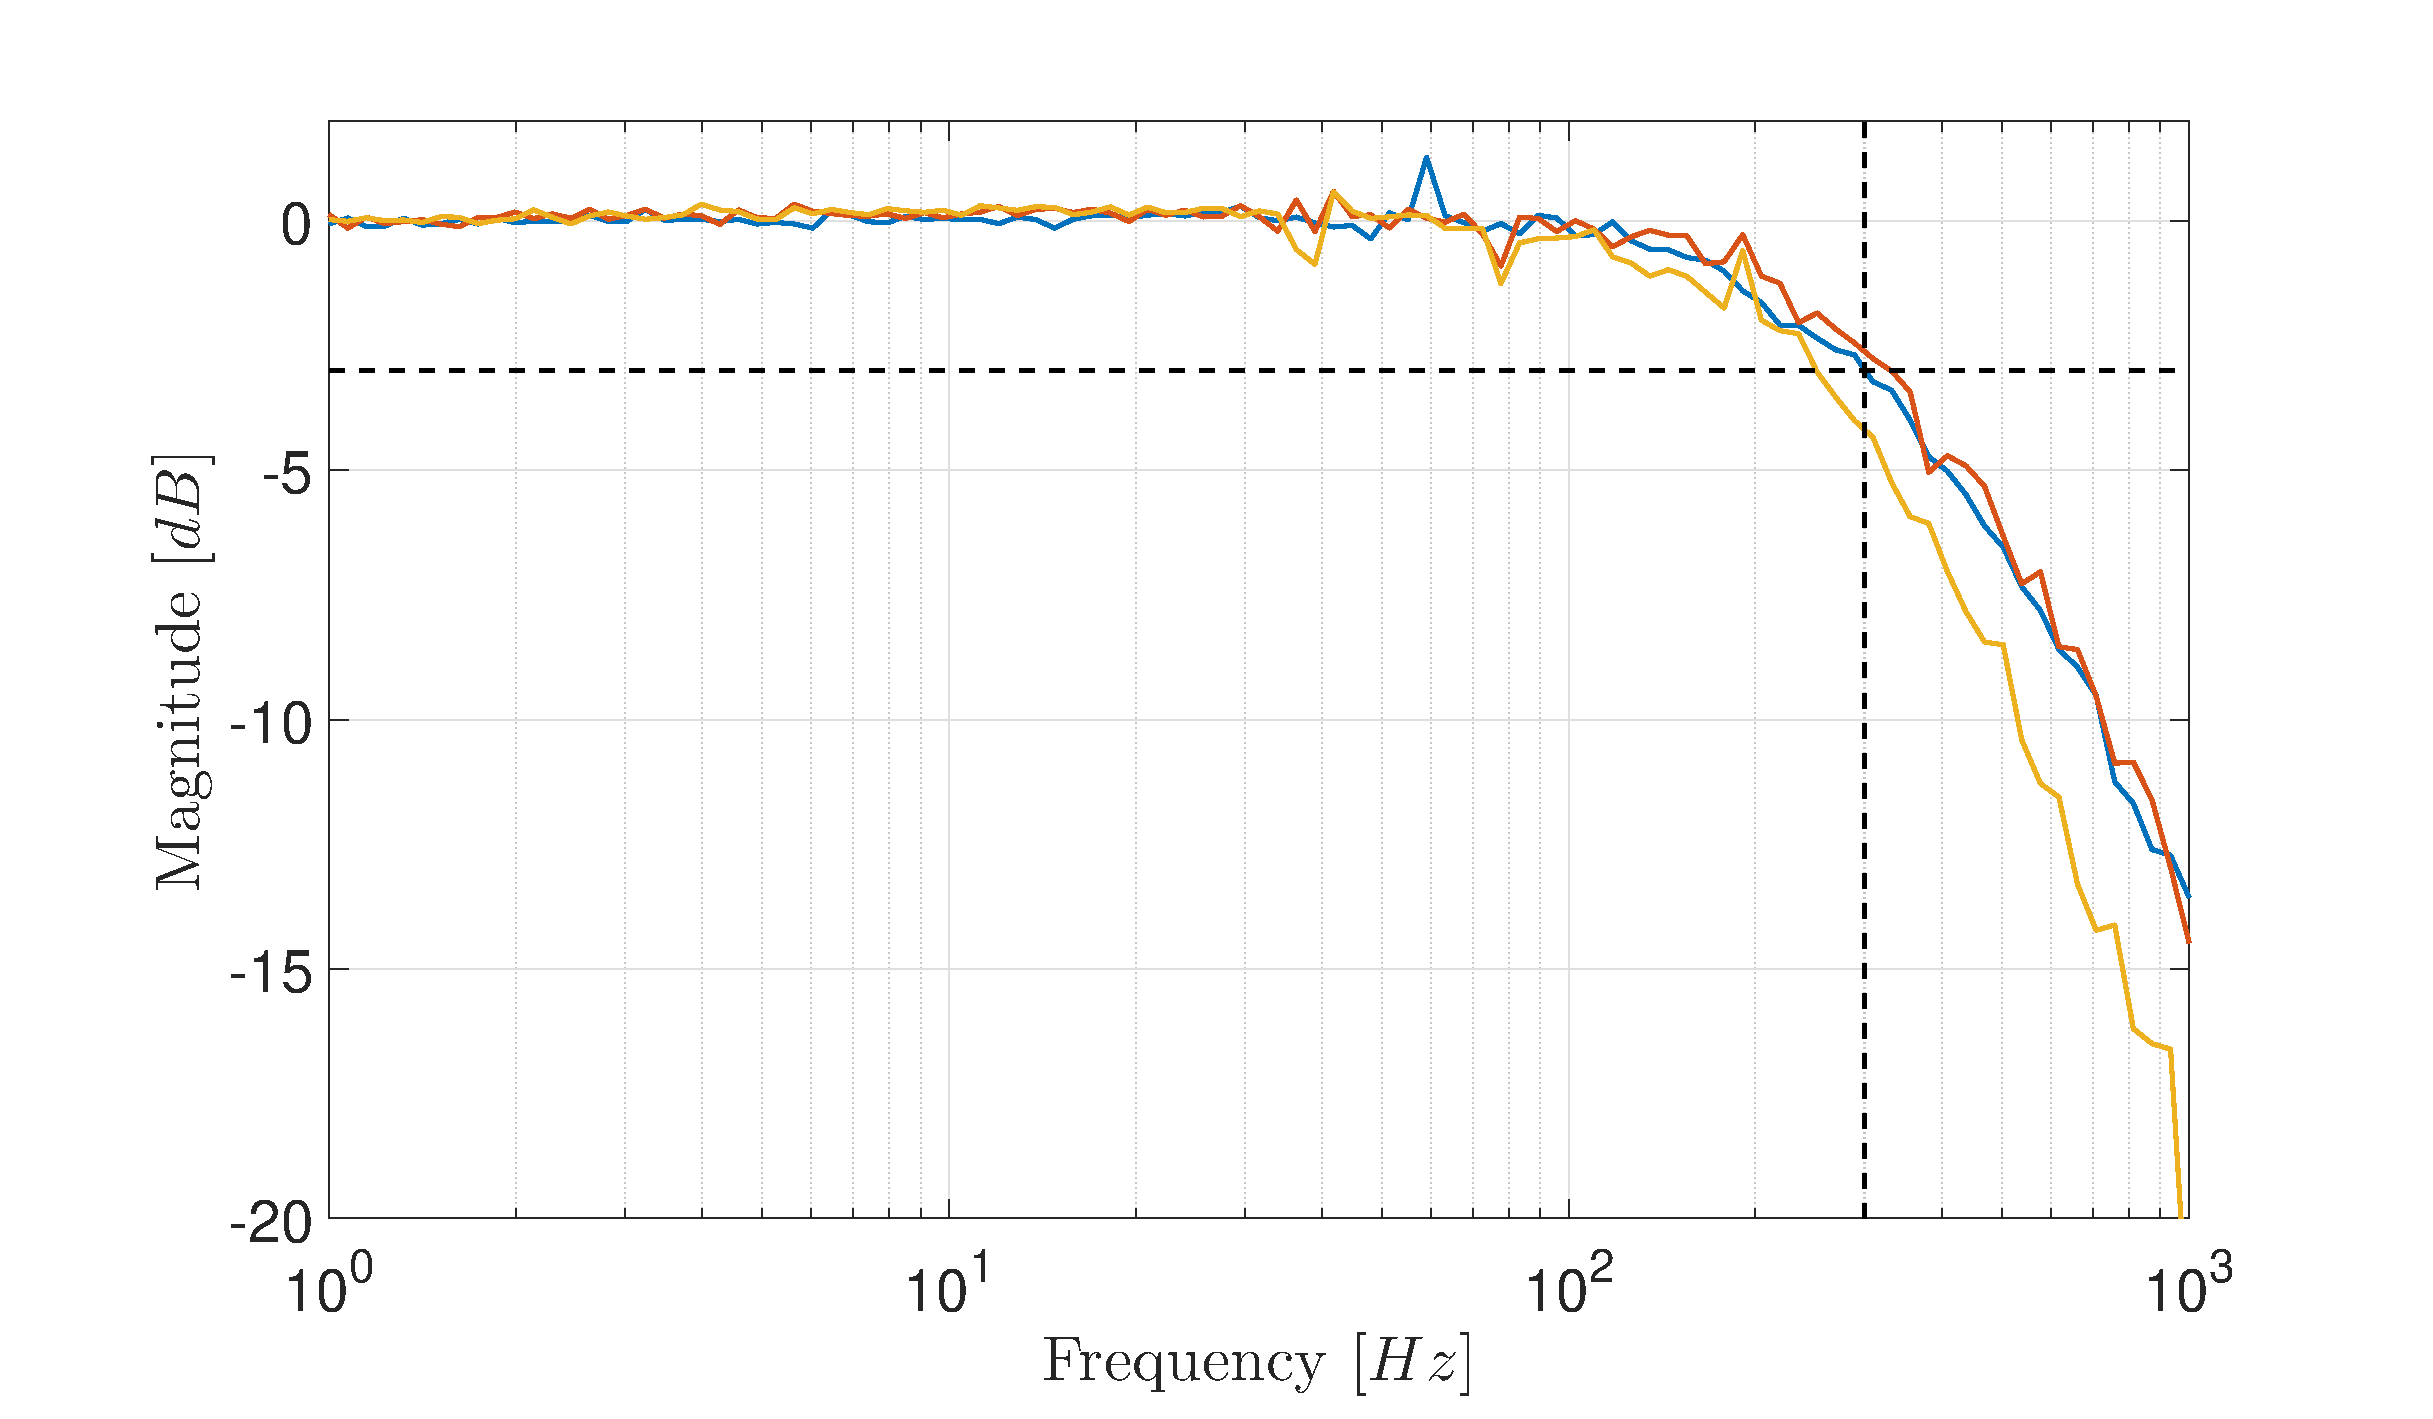
\includegraphics[width=\columnwidth]{../pics/d_loop_mag.eps}
\caption{The closed-loop response of $|T^{\prime}(j\omega)|$; data-driven method with $\mathcal{H}_{\infty}$ performance (red line); data-driven method with $\mathcal{H}_2$ performance (blue line); model-based approach with $\mathcal{H}_{\infty}$ performance (yellow line); $-3 \: dB$ point representing $300 \: Hz$ bandwidth (dashed-black line).}
\label{fig:d_loop}
\end{figure} 

\begin{figure}
\centering
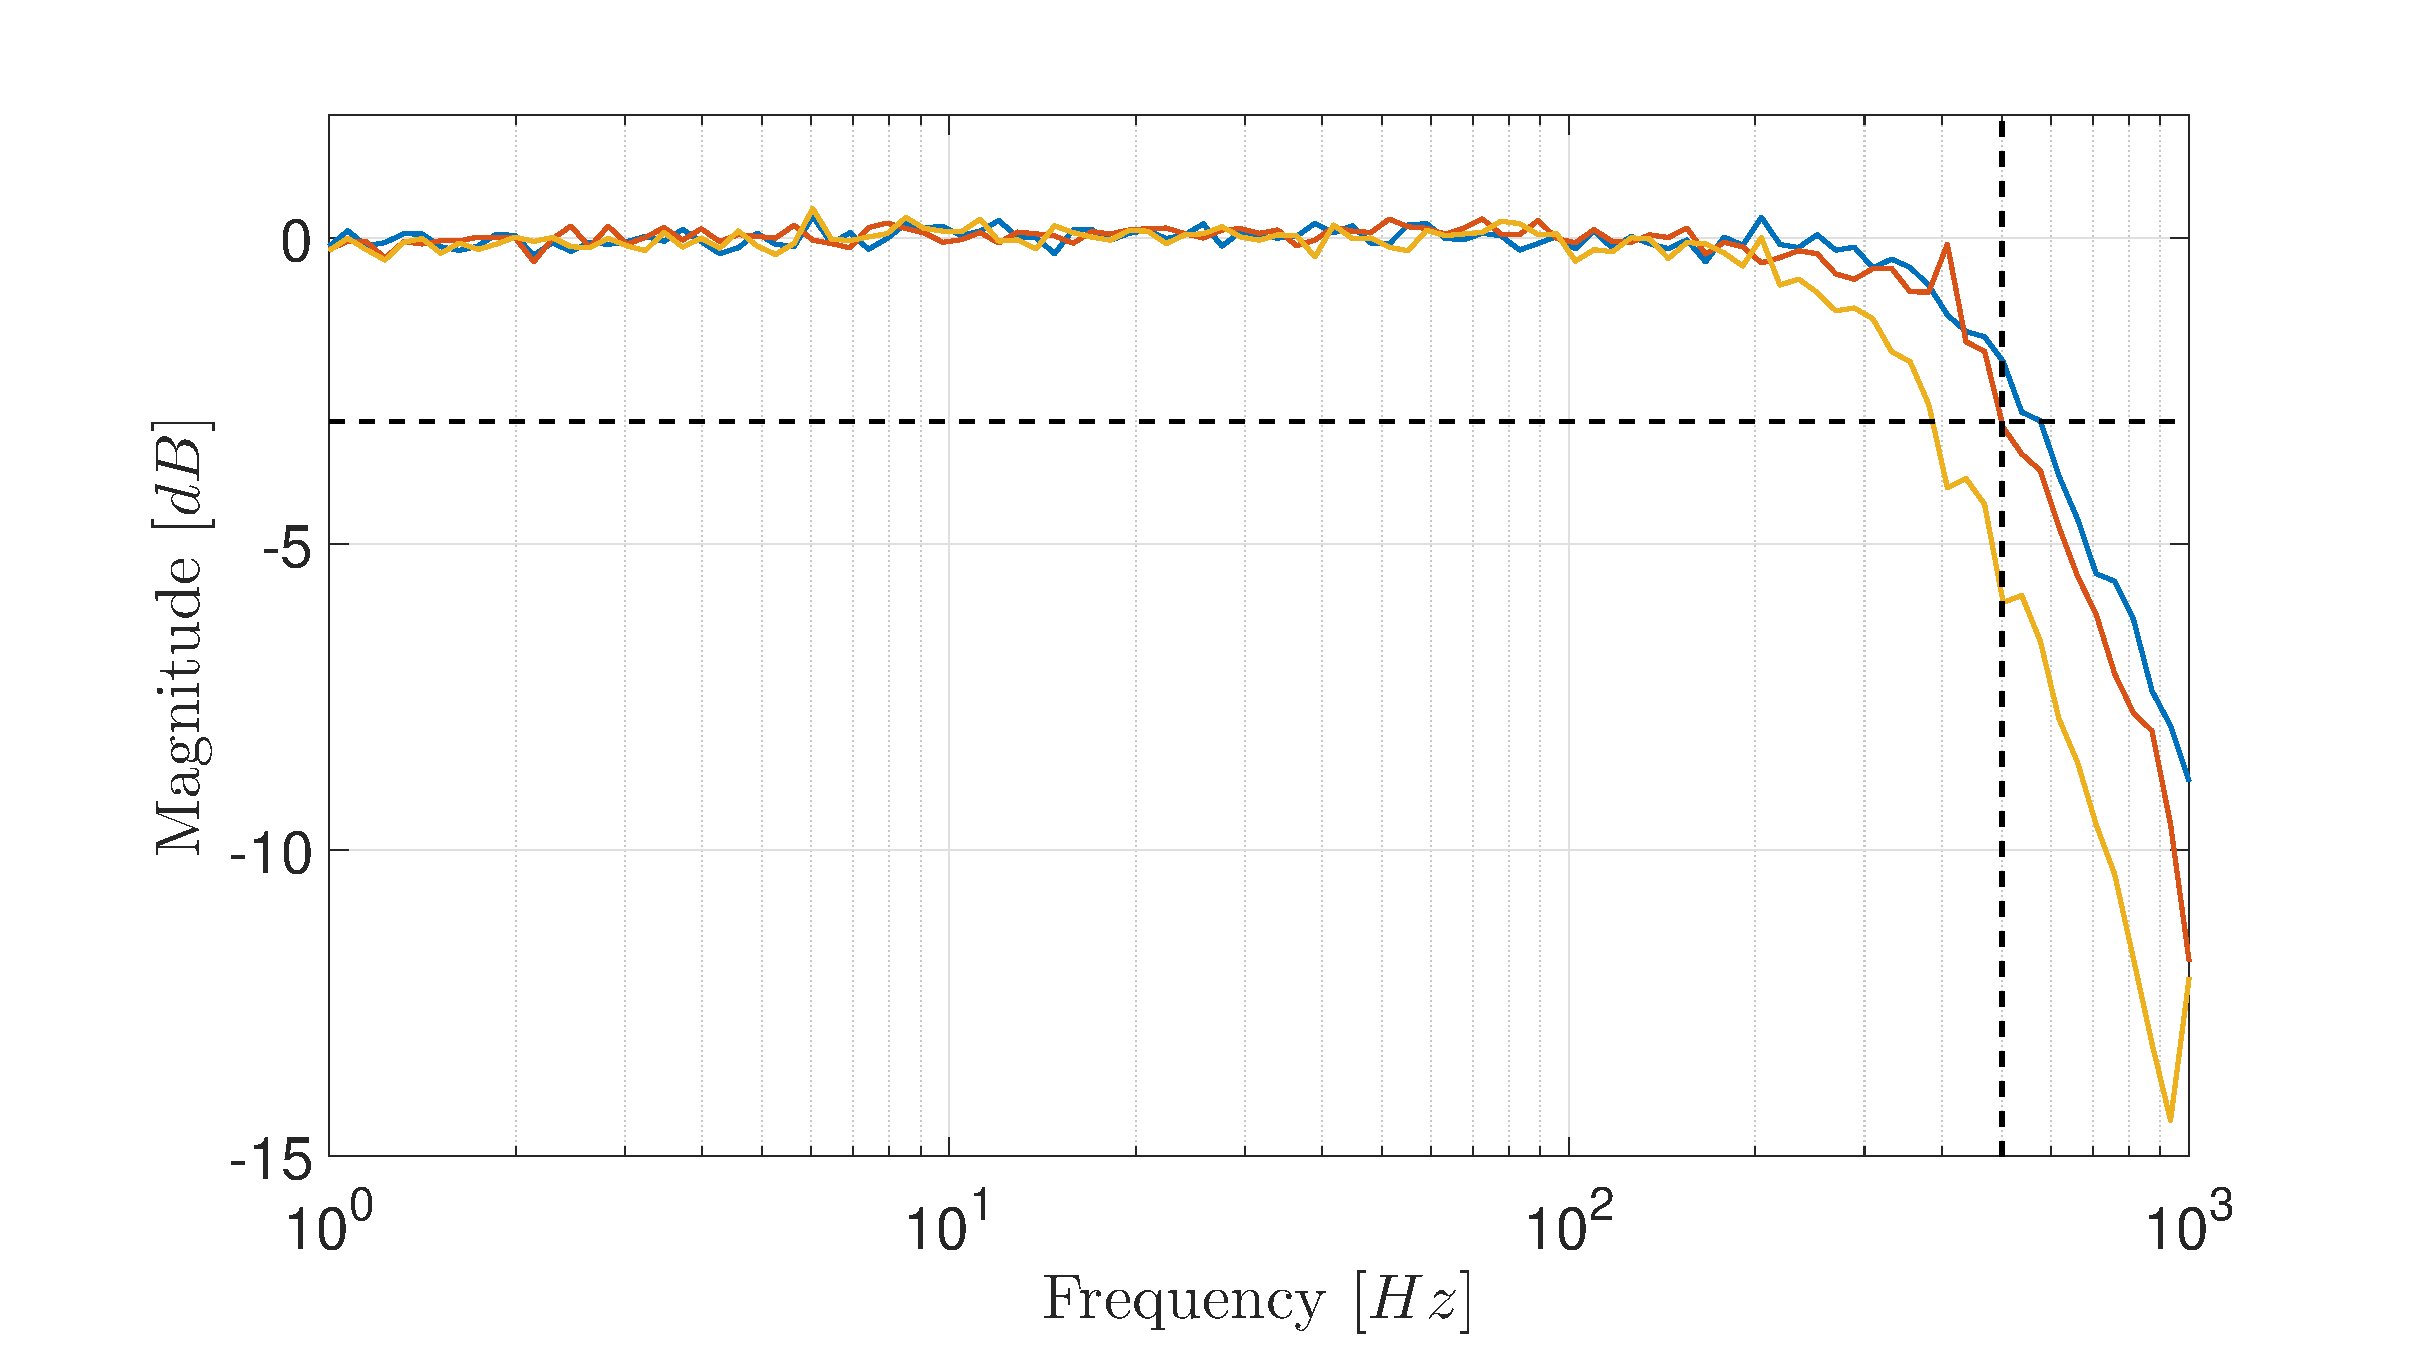
\includegraphics[width=\columnwidth]{../pics/v_loop_mag.eps}
\caption{The closed-loop response of $|T(j\omega)|$; data-driven method with $\mathcal{H}_{\infty}$ performance (red line); data-driven method with $\mathcal{H}_2$ performance (blue line); model-based approach with $\mathcal{H}_{\infty}$ performance (yellow line); $-3 \: dB$ point representing $500 \: Hz$ bandwidth (dashed-black line).}
\label{fig:v_loop}
\end{figure} 

\section{Conclusion}
\label{sec:conclusion}
A new data-driven method for computing a controller for the CERN power converter control system that attains $\mathcal{H}_2$ or $\mathcal{H}_{\infty}$ performance has been presented. A frequency-domain approach has been used in order to avoid the problem of unmodeled dynamics associated with parametric models. A non-convex loop-shaping constraint was convexified by linearizing the non-convex function around a stabilizing operating point. This linearization process allowed the use of the Shur Complement Lemma to construct an LMI and solve a convex optimization problem. This method has been applied to a power converter control system which uses a specific controller structure and is used for experimental purposes at CERN. In the case study presented in this paper, it has been shown that the proposed data-driven method offers a systematic optimization-based approach that meets the challenging specifications required for the application. In future work, it would be 


\bibliography{linear}
\end{document}